\renewcommand{\implies}{\Rightarrow}
\renewcommand{\impliedby}{\Leftarrow}
\newcommand{\V}{\ensuremath{\mathcal{V}}}
\newcommand{\At}{\ensuremath{\mathbb{A}}}
\newcommand{\T}{\ensuremath{\mathbb{T}}}
\newcommand{\tI}{\textbf{I}}
\newcommand{\tK}{\textbf{K}}
\newcommand{\tS}{\textbf{S}}
\newcommand{\tLambda}{\texorpdfstring{\ensuremath{\Lambda}}{Lambda}}
\newcommand{\tlambda}{\texorpdfstring{\ensuremath{\lambda}}{lambda}}
\newcommand{\talpha}{\texorpdfstring{\ensuremath{\alpha}}{alpha}}
\newcommand{\tbeta}{\texorpdfstring{\ensuremath{\beta}}{beta}}
\newcommand{\teta}{\texorpdfstring{\ensuremath{\eta}}{eta}}
\newcommand{\zB}{z.\,B. } 
\newcommand{\betared}{\ensuremath{\rightarrow_\beta}}
\newcommand{\msbetared}{\ensuremath{\twoheadrightarrow_\beta}}
\newcommand{\etared}{\ensuremath{\rightarrow_\eta}}
\newcommand{\msetared}{\ensuremath{\twoheadrightarrow_\eta}}
\newcommand{\etaexp}{\ensuremath{\rightarrow_\eta^{-1}}}
\newcommand{\msetaexp}{\ensuremath{\twoheadrightarrow_\eta^{-1}}}
\newcommand{\nat}{\ensuremath{\mathbb{N}}}
\newcommand{\IPCarr}{\ensuremath{\text{IPC}_\to}}
\newcommand{\STLC}{\ensuremath{\lambda_\to}}
\newcommand{\Long}{\text{Long}}
%\newcommand{\lam}{\ensuremath{\lambda}}


\chapter{Der einfach getypte Lambda-Kalkül}
\label{ch:stlc}

In diesem Kapitel werden die Grundlagen des einfach getypten Lambda-Kalküls ($\STLC$) vorgestellt, die wir in den späteren Kapiteln benötigen.
Der einfach getypte Lambda-Kalkül setzt sich aus den \tlambda-Termen und den einfachen Typen zusammen. Zunächst werden die Terme eingeführt, sowie eine Vorschrift, die es erlaubt Berechnungen über \tlambda-Terme durchzuführen. Des Weiteren werden Normalformen definiert, die insbesondere in den nachfolgenden Kapiteln wichtig werden.
 
Weiter werden die einfachen Typen eingeführt und diese mit den \tlambda-Termen kombiniert, um ein Typsystem zu erhalten und den Begriff der Inhabitation zu definieren und zu untersuchen.

Zuletzt werden wir eine alternative, aber äquivalente Definition der \tlambda-Terme kennenlernen, die es uns einfacher macht, computergestützt Aussagen über den einfach getypten Lambda-Kalkül aufzustellen und zu beweisen.
\section{\tlambda-Terme}
\tlambda-Terme sind eine Notation für funktionale Berechnungen. Wir werden zunächst \tlambda-Präterme betrachten und auf Basis derer die \tlambda-Terme definieren, die wir in diesem und dem nächsten Kapitel nutzen werden. Wir nutzen hier die Formalisierung aus \cite{lecturesCH}.
\begin{definition}{\tlambda-Präterm}{preterm}
    Sei \V{} eine abzählbar unendliche Menge an Variablensymbolen, dann sei die Menge $\Lambda^-$ der \emph{\tlambda-Präterme} die kleinste Menge mit den folgenden Eigenschaften.
\begin{align*}
    v\in\V&\implies v\in\Lambda^- & (\text{Variable})\\
    M, N \in\Lambda^-&\implies (M~N)\in\Lambda^- & (\text{Applikation})\\
    v\in\V\land M\in\Lambda^-&\implies (\lambda x.M)\in\Lambda^- & (\text{Abstraktion})
\end{align*}
\end{definition}
\begin{notation}
    Applikationen binden nach links und Abstraktionen nach rechts. Wir verzichten auf Klammerung, falls Zugehörigkeit über die Bindungsregeln eindeutig ist. Des Weiteren verzichten wir auf die äußerste Klammer eines Terms und fassen mehrere Abstraktionen zu einer zusammen.
    Anstelle der Terme \[(((M~N)~O)~P), (\lambda x.(\lambda y.x))\text{ und }((\lambda x.(P~Q))~R)\] schreiben wir
    \[M~N~O~P, \lambda x~y.x\text{ und }(\lambda x.P~Q)~R\].
\end{notation}
\begin{convention}
    Wir bezeichnen Terme üblicherweise mit Großbuchstaben aus der Mitte des Alphabets (\zB $M,N,P,Q$), und Variablen mit Kleinbuchstaben aus den letzten Buchstaben des Alphabets (\zB $x,y,z$).
\end{convention}
\begin{remark}
    Abstraktionen werden häufig anonyme Funktionen genannt. Anstelle eine Funktion direkt mit einem Namen zu definieren, wie beispielsweise $f(x) = x$, können wir mithilfe von \tlambda-Termen die Funktion unabhängig von ihrem Namen notieren. Selbstverständlich können wir den Term anschließend einen Namen zuweisen, $f = \lambda x.x$. Formal definieren wir dadurch nur die Berechnungsvorschrift einer Funktion, eine Funktion ist aber zusätzlich noch über ihren Definitions- und Wertebereich definiert. Wir werden diese Beobachtung in \Cref{sec:simpltypes} erneut betrachten.
\end{remark}
\begin{example}{}{}
\begin{itemize}
    \item Der Term $\lambda x.x$ entspricht der Funktion $f(x)=x$ und wird mit \tI{} abgekürzt.
    \item Der Term $\lambda x~y.x$ entspricht der Funktion $f(x, y)=x$ und wird mit \tK{} abgekürzt.
    \item Der Term $\lambda x~y~z.x~z~(y~z)$ entspricht der Funktion $f(x, y, z) = x(z)(y(z))$ und wird mit \tS{} abgekürzt.
    \item Der Term $x$ entspricht der Konstanten $x$. Hierbei ist zu bemerkten, dass wir Konstanten als nullstellige Funktionen auffassen können.
    \item Der Term $y~x$ entspricht $y(x)$ der Anwendung einer Funktion $y$ auf einen Term $x$.
\end{itemize}
\end{example}
\begin{remark}
    Die Terme \tS,\tK{} und \tI{} bilden die Grundlage des SKI-Combinator-Calculus.\cite{Schoenfinkel1924}    
\end{remark}

Wenn wir den Term $\lambda x.x$ und den Term $\lambda y.y$ betrachten, so entsprechen sie den Funktionen $f(x)=x$ und $f'(y)= y$. Es ist intuitiv klar, dass sich $f$ und $f'$ gleich verhalten. Sie nehmen eine Eingabe und geben diese unverändert zurück. Hierbei ist es unerheblich, ob die Eingabe $x$ oder $y$ genannt wird. Syntaktisch sind sie jedoch verschieden. Wenn wir rein die Konstruktion über die \tlambda-Präterme betrachten, folgt, dass $\lambda x.x \neq \lambda y.y$. 

Um diese intuitive Gleichheit zu formalisieren, führen wir zunächst Ersetzungen von Variablen in Termen ein. Darauf aufbauend werden zunächst wir eine Relation einführen, die nach unserer Intuition gleiche Terme in Relation setzt, also $\lambda x.x \sim \lambda y.y$, sowie einer Definition für \tlambda-Terme, in denen gilt $\lambda x.x = \lambda y.y$.
    
\subsection{Substitution}

Die Substitution ist die Grundlage des Berechnungsmodells im Lambda-Kalkül. Vereinfacht betrachtet ersetzen wir alle Variablen, die durch eine Abstraktion eingeführt werden durch einen Term, der durch die rechte Seite einer Applikation gegeben wird. Betrachten wir dazu zunächst, wie wir intuitiv einen \emph{Rechenschritt} mittels mathematischen Funktionen durchführen. Sei $f : \nat\to\nat$ eine Funktion, die mit $f(x) = x + 3$ definiert ist. Wollen wir nun $f(3)$ berechnen, ersetzen wir zunächst alle Vorkommen von $x$ durch $3$ und erhalten die nullstellige Funktion $3 + 3$, welche wir später weiter zu $6$ auswerten können.

Wir übertragen nun diese Intuition auf unsere \tlambda-Präterme. Sei $c_3$ ein \tlambda-Präterm, der der natürlichen Zahl $3$ entspricht und $A_+$ ein \tlambda-Präterm, der der (natürlichen) Addition entspricht\footnote{Die entsprechenden Terme existieren. Die Terme $c_n$ heißen Churchnumerale. Siehe hierfür \cite{lecturesCH}}, dann können wir den folgenden Term formulieren, der der Funktion $f$ entspricht \[\lambda x. A_+~x~c_3.\]


Wir können im \emph{inneren} \tlambda-Term alle $x$ durch $c_3$ ersetzen, um den Term $A_+~c_3~c_3$ zu erhalten. Wir schreiben $M[x/N]$ für den Term $M$, in dem die Variable $x$ durch den Term $N$ ersetzt wurde. Es gilt somit $(A_+~x~c_3)[x/c_3]=A_+~c_3~c_3$. Die Substitution verhält sich somit genau, wie unser intuitives Verständnis.

Aufpassen müssen wir bei geschachtelten Abstraktionen. Wir erinnern uns, dass in unserem intuitiven Verständnis gelten soll, dass $\lambda x.x\sim\lambda y.y$. Des Weiteren soll gelten, dass falls $M\sim N$ auch für alle $x$ und $P$ gelten soll, dass $M[x/P]\sim N[x/P]$. Betrachten wir die beiden Substitutionen $(\lambda x.x)[x/P]$ und $(\lambda y.y)[x/P]$. Wenn wir einfach alle Vorkommen von $x$ einer Variable durch $P$ ersetzen, erhalten wir die Terme $\lambda x.P$ und $\lambda y.y$. Klar ist, dass die Terme vor der Substitution intuitiv gleich sind, klar ist aber auch, dass $\lambda x.P$ und $\lambda y.y$ nicht zwangsweise gleich sind.
Um dies zu verhindern, müssen wir Abstraktionen besonders behandeln. Hierfür benötigen wir eine Definition von gebundenen und freien Variablen.
\begin{definition}{Freie Variable}{fv}
Sei $x\in\V$ und $M,N\in\Lambda^-$. Dann ist $FV:\Lambda^-\to\mathcal{P}(\V)$ mit 
\begin{align*}
FV(x) &= \{x\}\\
FV(M~N) &= FV(M)\cup FV(N)\\
FV(\lambda x.N) &= FV(M)\setminus \{x\}
\end{align*} eine Funktion, die einem Term seine freien Variablen zuweist.
Falls $y\in FV(M)$, nennen wir $y$ eine \emph{freie Variable} im Term $M$.
\end{definition}
Analog können wir die Menge der gebundenen Variablen definieren.
\begin{definition}{Gebundene Variable}{bv}
Sei $x\in\V$ und $M,N\in\Lambda^-$. Dann ist $BV:\Lambda^-\to\mathcal{P}(\V)$ mit
    \begin{align*}
    BV(x) &= \emptyset\\
    BV(M~N) &= BV(M)\cup BV(N)\\
    BV(\lambda x.N) &= BV(N)\cup\{x\}
    \end{align*} eine Funktion, die einem Term seine gebundenen Variablen zuweise.
    Falls $y\in BV(M)$, nennen wir $y$ eine \emph{gebundene Variable} im Term $M$.
\end{definition}
\begin{remark}
    Eine Variable kann gleichzeitig als freie und als gebundene Variable in einem Term vorkommen.
    \[x\in BV(x~\lambda x.x) \text{ und } x\in FV(x~\lambda x.x)\]
\end{remark}

\begin{definition}{Geschlossener Term}{closed}
    Ein Term $M$ ist geschlossen, wenn $FV(M)=\emptyset$.
\end{definition}

Wir könnten nun eine Substitution angeben, die genau die freien Variablen eines Term ersetzt. In unserem obigen Beispiel gelte dann folgendes.
\[(\lambda x.x)[x/N] = \lambda x.x \sim \lambda y.y = (\lambda y.y)[x/N]\]

Wir müssen zusätzlich noch darauf achten, dass eine Substitution keine bereits vorhandenen gebundenen Variablen als freie Variablen einführt. Betrachten wir dazu die Substitution \((\lambda x.y)[y/x] \). Wenn gelten soll, dass $\lambda x.y \sim \lambda z.y$, da auch die Funktionen $f(x) = y$ und $f'(z) = y$ identisch sind, gilt ebenfalls $(\lambda x.y)[y/x] \sim (\lambda z.y)[y/x]$, also $\lambda x.x\sim\lambda z.y$. 
Es ist auch klar, dass die Gleichheit $\lambda x.x = \lambda z.x$ nicht mit unserem intuitiven Verständnis übereinstimmt. Um zu verhindern, dass eine gebundende Variable als freie Variable in dem einzusetzenden Term vorkommt, können wir die gebundene Variable zuvor durch eine unbenutzte Variable ersetzen und damit eine Substitutionsvorschrift definieren, die unsere intuitive Gleichheit von Termen respektiert.

\begin{definition}{Frische Variable}{fresh}
    Eine Variable $x$ ist genau dann \emph{frisch} in einem Term $M$, wenn sie weder als freie, noch als gebundene Variable vorkommt.
\end{definition}
\begin{proposition}{}{fresh}
    Zu jedem Term $M$ gibt es unendlich viele Variablen, die frisch sind.
    \Proof Jeder Term $M$ ist endlich, damit ist die Menge der vorkommenden Variablen endlich. Eine Variablenmenge \V{} ist abzählbar unendlich.    
\end{proposition}
\begin{definition}{Substitution}{subst}
    Sei $M, P\in\Lambda^-$, $z\in\V$ frisch in $M$ und $P$, $x,y\in\V$ mit $x\neq y$. Wir definieren die \emph{Substitution} $M[x/P]$ durch Fallunterscheidung über $M$.
    \begin{align*}
    x[x/P] &= P\\
    y[x/P] &= y\\
    (M~N)[x/P] &= M[x/P]~N[x/P]\\
    (\lambda y.N)[y/P] &= \lambda y.N\\
    (\lambda x.N)[y/P] &=\begin{cases}
    \lambda z.N[x/z][y/P]& \text{Falls x}\in FV(P)\cap FV(N)\\
    \lambda x.N[y/P]& \text{sonst}
    \end{cases}
    \end{align*}
\end{definition}
\begin{remark}
    \begin{itemize}
        \item In der Literatur gibt es für die Substitution verschiedene Notationen. Wir folgen hier \cite{Troelstra1996}, sodass wir eine Substitution $[a/b]$ als das Ersetzen von $a$ durch $b$ lesen. Es gibt auch die Lesart, sodass wir $b$ durch $a$ ersetzen.\cite{curry}
    \item Es gibt aufgrund \Cref{prop:fresh} immer eine frische Variable $z$, die wir wählen können.
        \item Wir nennen eine Substitution durch eine Variable auch eine Umbenennung.
        \end{itemize}    
\end{remark}

Das folgende Lemma beweist die Intuition, dass falls eine Variable nicht in der Definition einer Funktion (frei) vorkommt, eine Ersetzung den Term nicht beeinflusst.

\begin{lemma}{}{freesubst}
    Für alle $x\in\V$, $M,N\in\Lambda$ gilt, falls $x\notin FV(M)$, dann gilt $M[x/P] = M$
    \Proof
    Durch Induktion über M.
    \begin{description}
        \item[Fall (IA) $M = y$:] 
        \[x\notin FV(y)\implies x \neq y \implies y[x/P] = y\]
        \item[Fall $M = P~Q$:]  
        \begin{align*}
        x\notin FV(P~Q)&\implies x \notin FV(P) \land x \notin FV(Q)\\
        &\overset{IH}{\implies} P[x/N] = P \land Q[x/N] = Q \\
        &\implies (P~Q)[x/N)=P~Q
        \end{align*}      
        \item[Fall $M = \lambda y.P$ und $x \neq y$:] 
        \begin{align*}
        &x\notin FV(\lambda y.P)\land x\neq y \\
        & \implies x\notin FV(P) \overset{IH}{\implies}P[x/N]=P\\
        &\implies \lambda y.P[x/N] = \lambda y.P \\
        &\implies (\lambda y.P)[y/N] = \lambda y.P
               \end{align*}        
        \item[Fall $M = \lambda x.N$:] 
        \[\lambda x.N[x/P]=\lambda x.N\]
    \end{description}
\end{lemma}

Wir können nun formulieren, dass zwei Terme in einer Art und Weise gleich sind, wenn sie sich nur in den Namen ihrer gebundenen Variablen unterscheiden.

\begin{definition}{\talpha-Äquivalenz}{alphaequiv}
    Seien $x,y\in\V$ Variablen, $N, N', M, M'\in\Lambda^-$ \tlambda-Präterme. Wir definieren die \talpha-Äquivalenz $\equiv_\alpha$ als kleinste transitive, reflexive und symmetrische Relation (Äquivalenzrelation) mit den folgenden Eigenschaften.
    \begin{align*}        
     \lambda x.M &\equiv_\alpha \lambda y.M[x/y]\\  
    M\equiv_\alpha M' \implies \lambda x.M &\equiv_\alpha \lambda x.M'\\
    M\equiv_\alpha M' \implies N~M&\equiv_\alpha N~M'\\
    N\equiv_\alpha N' \implies N~M&\equiv_\alpha N'~M.
    \end{align*}
\end{definition}

Mit der \talpha-Äquivalenz haben wir nun eine Relation für $\sim$, unter der die von uns als intuitiv gleich angesehenen Terme äquivalent sind. Dies können wir nun zu einem Begriff erweitern, der es uns erlaubt, diese äquivalenten Terme als gleich anzusehen.

\begin{definition}{\tlambda-Terme}{term}
    Sei $[M]_\alpha$ die Äquivalenzklasse des \tlambda-Präterms $M$ unter der Relation $\equiv_\alpha$, dann ist die Menge der \tlambda-Terme \tLambda{} definiert als
    \[\Lambda=\{[M]_\alpha\mid M\in\Lambda^-\}\]
\end{definition}
\begin{notation}
Wir werden implizit die Äquivalenzklasse weglassen, sodass wir anstelle $[\lambda x.x]_\alpha\in\Lambda$,
direkt $\lambda x.x\in\Lambda$ schreiben, es gilt somit $\lambda x.x = \lambda y.y$.
\end{notation}
\begin{remark}
    In der Literatur werden \tlambda-Terme häufig wie unsere \tlambda-Präterme definiert und anstelle der Gleichheit zwischen Termen wird nur eine Äquivalenz unter der \talpha-Äquivalenz angegeben. Unsere explizite Unterscheidung zwischen $\Lambda$ und $\Lambda^-$ erlaubt es uns echte Gleichheiten zwischen \tlambda-Termen für unser intuitives Verständnis von Gleichheit zu verwenden. Siehe hierzu auch \cite{lecturesCH}.
\end{remark}

Das folgende Lemma erlaubt es uns, die Reihenfolge von Substitutionen zu ändern.

\begin{lemma}{Substitutionslemma}{subst}
    Seien $M, N, P\in\Lambda$ \tlambda-Terme, $x, y\in\V$ Variablen mit $x\neq y$ und $x\notin FV(P)$, dann gelte :
    \[M[x/N][y/P]=M[y/P][x/N[y/P]]\]
    \Proof
    Siehe \cite{lecturesCH}.
\end{lemma}


\subsection{\tbeta-Reduktion}
Wir können mittels \tlambda-Termen nun Funktionen und Funktionsanwendungen notieren, haben aber noch keine Vorschrift, nach der wir Berechnungen ausführen können. Genauer fehlt uns eine Vorschrift, die eine Applikation einer Abstraktion und einen anderen Term zusammenführt. Betrachten wir erneut mathematische Funktionen. Wenn wir eine einstellige Funktion $f(x) = M$ haben und zu einen zu $f$ \emph{passenden}\footnote{Wir werden in \Cref{sec:simpltypes} uns damit befassen, was es bedeutet, dass ein Wert \emph{passend} für einen Term ist.} Wert $N$, können wir die Anwendung von $f$ auf $N$, also $f(N)$ berechnen, indem wir in $M$ alle $x$ durch $N$ substituieren. In den \tlambda-Termen entspräche dies einem Übergang von $(\lambda x.M)~N$ zu $M[x/N]$. 

\begin{definition}{Redex}{redex}
    Sei $x\in\V$ eine Variable und $M, N\in\Lambda$ zwei \tlambda-Terme. Wir nennen einen Term in der Form $(\lambda x.M)~N$ einen Redex.
\end{definition}

\begin{definition}{\tbeta-Reduktion}{betared}
    Sei $x\in\V$, $M, N, M', N'\in\Lambda$, dann definieren wir die \tbeta-Reduktion $\betared$ als kleinste Relation mit den folgenden Eigenschaften.
    \begin{align*}
    (\lambda x.M)~N&\betared M[x/N]\\
    M\betared M' \implies \lambda x.M&\betared \lambda x.M'\\
    M\betared M' \implies  M N&\betared M'~N\\
    N\betared N' \implies  M N&\betared M~N'    
    \end{align*}
\end{definition}
\begin{remark}
    Die \tbeta-Reduktion ersetzt genau einen Redex in einem Term. Der transitiv-reflexive Abschluss der \tbeta-Reduktion \msbetared, die sogenannte \emph{multi-step \tbeta-Reduktion}, ersetzt beliebig viele Redexe -- auch keinen -- in einem Term.
\end{remark}
Über die \tbeta-Reduktion können wir nun Rechnungen durchführen. Es ist sogar so, dass durch diese Relation der Lambda-Kalkül \emph{Turingvollständig} ist \cite{churchturing}\footnote{Der Lambda-Kalkül ist sogar älter als das Konzept der Turingmaschine. Vor der Einführung der Turingmaschine wurde Berechenbarkeit als \tlambda-Definierbarkeit über den Lambda-Kalkül definiert\cite{churchturing}.}. Wir werden in \Cref{ssec:nf} das Konzept \emph{Reduktion als Berechnung} aufgreifen und beschreiben, wann eine solche Berechnung terminiert.
\begin{example}{}{}
    \begin{itemize}
        \item $(\lambda x~y.x)~z\betared (\lambda y.x)[x/z] = \lambda y.x[x/z] = \lambda y.z$
        \item $(\lambda x.x~y)~(\lambda x.x)\betared (x~y)[x/\lambda x.x]= (\lambda x.x)~y \betared x[x/y]=y$
    \end{itemize}
\end{example}
\subsection{\teta-Reduktion}
Zwei weitere Relation, die wir einführen, sind die \teta-Reduktion und die \teta-Expansion. Die Grundidee hierbei ist es, \emph{unnötige} Abstraktionen zu vermeiden, bzw. explizit einen Term in eine weitere Abstraktion einzubetten. Wenn wir eine Abstraktion haben, die ihre abstrahierte Variable nur an ihren inneren Term weitergibt, können wir die Abstraktion auch weglassen, ohne das Verhalten des Terms zu ändern. Andersherum können wir jeden Term auch in zusätzliche Abstraktionen einbetten.
\begin{example}{}{eta}
    Betrachten wir den Term $(\lambda x.N~x)~M$ mit $x\notin FV(N)$. Nach den Regeln der \tbeta-Reduktion gilt $(\lambda x.N~x)~M\betared (N~x)[x/M] = N M$, jedoch gilt nicht $\lambda x.N x \betared N$. 
\end{example}
Es liegt nun nahe, dass $\lambda x.N x$ und $N$ aus \Cref{ex:eta} in einer geeigneten Relation zueinander stehen.
\begin{definition}{\teta-Reduktion}{etared}
    Sei $x,z\in\V$ eine Variable und $M,N\in\Lambda$ ein \tlambda-Term. Sei weiter $z\notin FV(N)$, dann definieren wir die \emph{\teta-Reduktion} $\etared$ als kleinste Relation mit den folgenden Eigenschaften.
    \begin{align*}
    \lambda z.N~z &\etared N\\
    M\etared M' \implies \lambda x.M&\etared \lambda x.M'\\
    M\etared M' \implies  M N&\etared M'~N\\
    N\etared N' \implies  M N&\etared M~N'        
    \end{align*}
\end{definition}
Analog dazu lässt sich die \teta-Expansion definieren.
\begin{definition}{\teta-Expansion}{etaexp}
    Sei $x,z\in\V$ eine Variable und $M,N\in\Lambda$ ein \tlambda-Term. Sei weiter $z\notin FV(N)$, dann definieren wir die \emph{\teta-Expansion} $\etaexp$ als kleinste Relation mit den folgenden Eigenschaften.
    \begin{align*}
    N &\etaexp \lambda z.N~z\\
    M\etaexp M' \implies \lambda x.M&\etaexp \lambda x.M'\\
    M\etaexp M' \implies  M N&\etaexp M'~N\\
    N\etaexp N' \implies  M N&\etaexp M~N'        
    \end{align*}
\end{definition}
\begin{remark}
    Analog zur \tbeta-Reduktion sind $\msetared$ und $\msetaexp$ die transitiv-reflexive Abschlüsse der \teta-Reduktion und \teta-Expansion.
\end{remark}
\subsection{Normalformen}
\label{ssec:nf}
Aufbauend auf den eingeführten Reduktionsregeln können wir nun Normalformen einführen, also Formen, in den die jeweilige Reduktion nicht mehr anwendbar ist. Wenn ein Reduktionsschritt ein Berechnungsschritt ist, ist eine Normalform das Ergebnis der Berechnung.

\begin{definition}{\tbeta-Normalform}{betanf}
    Ein Term $M$, zu dem es keinen Term $N$ gibt, sodass $M\betared N$, ist in \tbeta-Normalform.
\end{definition}

\begin{remark}
    Es gibt \tlambda-Terme, die keine \tbeta-Normalform haben, also deren Berechnung nicht terminiert. Dies ist insbesondere ein wichtiges Kriterium für die Turingvollständigkeit des Lambda-Kalküls. Betrachten wir den Term $\Omega = (\lambda x. x~x)~(\lambda x.x~x)$. Der Term enthält einen Redex, somit lässt er sich \tbeta-reduzieren. Eine Reduktion führt jedoch direkt wieder zu dem Term $\Omega$
    \begin{align*}
        \Omega&=(\lambda x.x~x)~(\lambda x.x~x)\betared (x~x)[x/\lambda x.x~x] \\&= x[x/\lambda x.x~x]~x[x/\lambda x.x~x]=(\lambda x.x~x)~(\lambda x.x~x)\\&=\Omega
    \end{align*}    
\end{remark}
\begin{remark}
Terme, die mehrere Redexe haben, stehen mit mehreren verschiedenen \tlambda-Termen gemäß der \tbeta-Reduktion in Relation. Die \tbeta-Reduktion ist somit nicht eindeutig.
\end{remark}

Auch zu der \teta-Reduktion können wir einen Normalformbegriff definieren. 

\begin{definition}{\teta-Normalform}{etanf}
    Ein Term $M$, zu dem es keinen Term $N$ gibt, sodass $M\etared N$ ist in \teta-Normalform.
\end{definition}

Wir werden in \Cref{longnf} eine Art Normalformbegriff für die \teta-Expansion kennenlernen.

\begin{figure}
    \center
    \begin{tikzpicture}[node distance=2cm]
    \node (M) at (0,0) {$M$};
    \node (P) [below left of = M] {$P$};    
    \node (Q) [below right of = M] {$Q$};
    \node (Z) [below right of = P] {$Z$};
    \path[draw, ->>] (M) -> (P);
    \path[draw, ->>] (M) -> (Q);
    \path[draw, dashed , ->>] (Q) -> (Z);        
    \path[draw, dashed , ->>] (P) -> (Z);        
    \end{tikzpicture}
    \caption{Diamanteigeschaft}
    \label{fig:diamond}    
\end{figure}

Im Folgenden werden Wir feststellen, dass es für das Ergebnis der Berechnung eines \tlambda-Terms unerheblich ist, in welcher Reihenfolge wir Redexe auflösen. Zunächst führen wir eine Eigenschaft ein, die besagt, dass die Wahl des Abzuleitenden Subterms in einer Reduktion in der Hinsicht nicht relevant ist, dass wir immer zu einem gemeinsamen Ergebnisterm gelangen können.

\begin{definition}{Diamanteigenschaft}{diamond}
    Seien $M,P,Q\in\Lambda$ \tlambda-Terme, dann sagen wir, dass eine transitiv-reflexive Relation $\twoheadrightarrow$ die Diamanteigenschaft erfüllt oder konfluent ist, wenn
    \[M\twoheadrightarrow P \land M\twoheadrightarrow Q\implies \exists Z\in\Lambda. P\twoheadrightarrow Z \land Q\twoheadrightarrow Z. \]
    Siehe hierfür auch \Cref{fig:diamond}.
\end{definition}
\begin{proposition}{Church-Rosser}{diamond}
    $\msbetared$ und $\msetared$ erfüllen die Diamanteigenschaft.
    \Proof
%    Grundsätzlich gilt, wenn $M$ in Normalform ist, muss $M = P = Q$ gelten. Damit existiert ein $Z$ mit $Z = P = Q = M$.
%    \begin{enumerate}
%        \item Induktion über $M$.
%        \begin{description}
%            \item[Fall $M=x$:] $x$ ist in Normalform.
%            \item[Fall $M=\lambda x.N$:] $P$ und $Q$ müssen in der Form $\lambda x.P'$ und $\lambda x.Q'$ mit $N\msbetared P'$ und $N\msbetared Q'$ sein. Nach Induktionshypothese gibt es ein $Z'$, sodass $P'\msbetared Z'$ und $Q'\msbetared Z'$. Somit gilt auch $P\msbetared \lambda x.Z'$ und $Q\msbetared \lambda x.Z'.$
%            \item[Fall $M=S~T$:] Hier unterscheiden wir 2 Fälle. $M$ selbst ist ein Redex oder ein Subterm von $S$ bzw. $T$ ist ein Redex, aber $M$ selbst nicht.
%            \begin{description}
%                \item[$M$ ist ein Redex] 
%            \end{description}
%        \end{description}
%        Fall M = x:
%
%        Fall $M = \lambda x.N$:
%          
%        Fall M = P'~Q':
%          
%    \end{enumerate}
Siehe \cite{lecturesCH}.
\end{proposition}     

Dies können wir nun erweitern, um festzustellen, dass eine Normalform -- also ein Ergebnis einer Berechnung -- nicht davon abhängt, in welcher Reihenfolge Redexe ausgewertet werden.

\begin{lemma}{Eindeutigkeit von Normalformen}{nfuniq}
    Seien $N_1$ und $N_2$ zwei Normalformen eines Terms $M$ zu einer Relation, dessen transitiv-reflexiver Abschluss die Diamanteigenschaft erfüllt, dann ist $N_1 = N_2$.
    \Proof
    Folgt direkt aus der Diamanteigenschaft. Ein Term in Normalform steht nur mit sich selbst in Relation, also $N_1 \twoheadrightarrow Z \implies Z = N_1$ und $N_2 \twoheadrightarrow Z \implies N_2 = Z$. Daher gilt $Z = N_1 = N_2$.
\end{lemma}
\section{Einfache Typen}
\label{sec:simpltypes}
Betrachten wir erneut Funktionen. Funktionen sind üblicherweise nicht nur durch ihren Funktionsrumpf definiert, sondern auch durch ihren Definitionsbereich (Domain) und Wertebereich (Codomain). Eine vollständige Definition für eine Funktion wäre die folgende:
\begin{align*}
f&:\nat\to\nat\\
f(x) &= x + 3
\end{align*}
Wir können hier $\nat\to\nat$ als Typ für die Funktion $f$ sehen. Die Menge der natürlichen Zahlen ist dann ein Typ für die Eingabe $x$ sowie für alle Ergebnisse von $f$. Betrachten wir den Aufbau des Typen $\nat\to\nat$. Dieser besteht aus zwei Komponenten, ein zweistelliger Operator $\to$ und die atomaren Typen $\nat$. 

Wir können ebenfalls der Identitätsfunktion $id(x) = x$ einen Typen geben. Die Domain und Codomain von $id$ ist durch die Definition nicht gegeben, es ist jedoch klar, dass die Codomain zumindest die Domain enthalten muss. Sei die Domain vom $id$ eine beliebige Menge $A$, so ist die Codomain mindestens eine Menge $B$ mit $A\subseteq B$. Insbesondere gilt $id : A \to A$. Dieses Prinzip können wir auf \tlambda-Terme erweitern. Es gibt es viele Typsysteme, die den Lambda-Kalkül typen, wir betrachten hier die einfachen Typen.
\begin{definition}{Einfache Typen}{simpletypes}
    Sei \At{} eine abzählbar unendliche Menge an Typatomen, dann ist die Menge \T{} der einfachen Typen definiert als kleinste Menge mit den folgenden Eigenschaften:
    \begin{align*}
    a\in\At&\implies a\in\T\\
    \alpha, \beta\in \T&\implies \alpha\to\beta\in\T
    \end{align*}
 \end{definition}
\begin{convention}
Wir bezeichnen Typen mit kleinen griechischen Buchstaben (\zB $\alpha,\beta$ aber auch $\sigma, \tau, \rho$), Typatome mit kleinen Buchstaben aus den ersten Buchstaben des Alphabets (\zB $a,b,c$)
\end{convention}
\begin{definition}{Teiltyp}{subformula}
    Sei $\rho\in\T$ ein einfacher Typ, dann ist die Menge $\text{codom}(P_\rho)$ seiner Teiltypen folgendermaßen induktiv definiert.
    \begin{align*}
        \text{codom}(P_b) &= b &\text{für }b\in\At\\
        \text{codom}(P_{\sigma\to\tau}) &= 
        \begin{aligned}[t]
         &\{\sigma\to\tau\}~\cup\\
         &\text{codom}(\sigma)~\cup\\
         &\text{codom}(\tau)
        \end{aligned}
    \end{align*}
    
    Falls $\rho'\in\text{codom}(\rho)$, aber $\rho \neq \rho'$, dann nennen wir $\rho'$ einen echten Teiltypen von $\rho$.
\end{definition}
\begin{remark}
    \begin{itemize}
        \item Die Benennung der Menge der Teiltypen deutet bereits an, dass $P_\rho$ eine Funktion darstellt. Dies ist der Fall und sie wird in \Cref{def:path} definiert.
        \item In der Literatur wird anstelle von Teiltypen auch von Subformelen gesprochen. Dies hängt mit dem \emph{Curry-Howard-Isomorphismus} zusammen, der besagt, dass Typen Formeln darstellen. Wir werden dies in \Cref{sec:IPC} betrachten.
    \end{itemize}
\end{remark}
Analog zu den Variablen in \tlambda-Termen können wir für Typatome in einfachen Typen eine Definition für unbenutzte, frische Variablen aufstellen.
\begin{definition}{Frisches Typatom}{freshat}
    Wir nennen ein Atom $a$ \emph{frisch} in einem Typen $\rho$, wenn es nicht als Teiltyp von $\rho$ auftaucht.
\end{definition}
\section{Typisierung}
Wir benötigen nun einen Kalkül, mit dem wir Terme und Typen in Relation setzen können. Es ist auffällig, dass $\lambda x.M$ eine (mindestens einstellige) Funktion darstellt und $\alpha\to\beta$ ein Funktionstyp ist. Interpretieren wir $\alpha$ als Domain und $\beta$ als Codomain der Funktion, müssen alle Terme $N$, auf die die Funktion angewendet wird, den Typen $\alpha$ haben und der Term $M[x/N]$ den Typen $\beta$.
Da $N$ den Typen $\alpha$ hat, muss $x$ in $M$ auch den Typen $\alpha$ haben. Wir müssen uns also merken, dass in $M$ die Variable $x$ mit $\alpha$ getypt wird. Dazu müssen wir uns einen Typkontext merken, der Variablen Typen zuweist. Wir führen hierfür eine Relation $\Gamma\vdash M:\rho$ ein, die aussagt, dass zu einem Typkontext $\Gamma$ der Term $M$ mit dem Typen $\rho$ getypt werden kann.

\begin{definition}{Typkontext}{context}
    Ein Typkontext $\Gamma$ ist eine Relation mit $\Gamma\subseteq \V\times\T$, bei der alle Elemente aus $\V$ maximal einmal in der Domain der Relation vorkommen dürfen.
\end{definition}
\begin{notation}
    Wir schreiben Elemente $(x,\rho)$ aus $\Gamma$ als $x : \rho$. Des Weiteren schreiben wir $\Gamma, x:\rho$ anstelle von $\Gamma\cup(x,\rho)$. Hierbei ist zu beachten, dass die Bedingung an Typkontexte nicht verletzt wird, da durch das Hinzufügen eine Variable mit mehreren Typen getypt werden könnte.
\end{notation}

\begin{definition}{Typisierung}{typing}
    Seien $\Gamma\subseteq\V\times\T$ ein Typkontext, $\sigma,\tau,\rho\in\T$ einfache Typen, $M, N\in\Lambda$ \tlambda-Terme und $x\in\V$ eine Variable. Wir definieren die Typisierung $\_ \vdash \_ : \_$ anhand folgender Inferenzregeln.
  \[\infer[\var]{\Gamma,x:\rho\vdash x : \rho}{}\]
  \[\infer[\abs]{\Gamma\vdash\lambda x.M : \sigma\to\tau}{\Gamma, x:\sigma\vdash M:\tau}\]
  \[\infer[\app]{\Gamma\vdash M~N :\tau}{\Gamma\vdash M : \sigma\to\tau&\Gamma\vdash N : \sigma}\]
  
  Wir bezeichnen einen Baum $\mathcal{D}$ mit Wurzel $\Gamma\vdash M : \rho$, der sich durch die Anwendung der obigen Inferenzregeln ergibt, als Typableitung. Wenn $\mathcal{D}$ die Typableitung zu der Typisierung $\Gamma\vdash M : \rho$ ist, schreiben wir auch $\mathcal{D}\judges\Gamma\vdash M:\rho$.
  
\end{definition}
\begin{notation}
    Anstelle von $\emptyset\vdash M : \rho$ schreiben wir auch $\vdash M:\rho$.
\end{notation}

Jede Art, einen \tlambda-Term $M$ zu konstruieren, korrespondiert zu genau einer Typisierungsregel. Betrachten wir den äußersten Konstruktor von $M$, lässt sich ablesen, welche Regel genutzt wurde, um $M$ zu typen. Dies wird im folgenden Generierungslemma formalisiert.

\begin{lemma}{Generierungslemma}{simplgen}
    Sei $\Gamma\subseteq\V\times\T$ ein Typkontext, $M\in\Lambda$ ein \tlambda-Term und $\rho\in\T$ ein einfacher Typ. Gelte weiter $\Gamma\vdash M:\rho$. Dann gilt
    \begin{itemize}
        \item falls $M = x$, $x : \rho\in\Gamma$
        \item falls $M = \lambda x.N$, $\rho = \sigma\to\tau$ sodass $\Gamma, x:\sigma\vdash N:\tau$
        \item falls $M = P~Q$, es existiert ein $\sigma$, sodass $\Gamma\vdash M:\sigma\to\rho$ und $\Gamma\vdash N:\sigma$
    \end{itemize}
    \Proof
    In jedem Beweisschritt ist es eindeutig, welche Regel gewählt wird. 
\end{lemma}

\begin{definition}{Typbar}{typable}
Terme, zu denen es ein $\Gamma$ und ein $\rho$ gibt, sodass $\Gamma\vdash M : \rho$, nennen wir typbar.
\end{definition}

\begin{example}{}{typable}
    \begin{enumerate}
        \item Der Term $\tI$ ist typbar mit $\vdash\tI:\alpha\to\alpha$
        \item Der Term $x~x$ ist nicht typbar. 
    \end{enumerate}
\Proof
\begin{enumerate}
      \item \[
    \infer[(abs)]{\vdash \lambda x.x:\alpha\to\alpha}{\infer[(var)]{x:\alpha\vdash x : \alpha}{}}
    \]
    \item Es ist klar, dass $x~x$ in einem Kontext, der nicht $x$ enthält, nicht typbar ist. Nehmen wir an, dass es eine Typisierung $\Gamma,x:\alpha\vdash x~x:\rho$ gibt. Laut \Cref{lem:simplgen} gibt es ein $\sigma$, sodass $\Gamma, x:\alpha\vdash x:\sigma\to\rho$ und $\Gamma, x:\alpha\vdash x:\sigma$.
    
    Weiter folgt nach \Cref{lem:simplgen}, dass $\alpha=\sigma=\sigma\to\rho$ gelten muss. Die Gleichung $\sigma = \sigma\to\rho$ kann für endliche Typen nicht erfüllt werden, und \Cref{def:simpletypes} erlaubt nur endliche Typen.	    
    \end{enumerate}
\end{example}

\begin{lemma}{Subtypbar}{subtypable}
    Sei $M\in\Lambda$ ein \tlambda-Term, der typbar ist. Dann ist jeder Subterm von $M$ ebenfalls typbar.
    \Proof
    Folgt direkt aus \Cref{lem:simplgen}.
\end{lemma}

\begin{definition}{Inhabitanten}{inhab}
    Falls $\vdash M:\rho$, nennen wir $M$ einen Inhabitanten von $\rho$ und $\rho$ inhabitiert.
\end{definition}

\begin{lemma}{Subject-Reduction}{subjred}
    Falls $\Gamma\vdash M:\rho$ und $M \msbetared N$, dann $\Gamma\vdash N:\rho$.
    \Proof
    Siehe \cite{lecturesCH}.    
\end{lemma}
\begin{remark}
    Die umgekehrte Richtung gilt nicht. Betrachten wir die Terme $\tI$ und $\tK~\tI~\Omega$. Es gilt $\tK~\tI~\Omega\betared\tI$ und $\vdash \tI:\alpha\to\alpha$, es gilt jedoch nicht, dass $\vdash\tK~\tI~\Omega:\alpha\to\alpha$. Es ist sogar so, dass $\tK~\tI~\Omega$ nicht typbar ist, da $x~x$ ein Subterm von $\Omega$ ist und $x~x$ nicht typbar ist. Siehe \Cref{lem:subtypable} und \Cref{ex:typable}.
\end{remark}

\begin{definition}{Typsubstitution}{typesubst}
Eine Funktion $Su : \At\to\T$ nennen wir Typsubstitution. 
Wir können eine Substitution $Su$ zu einer Funktion $Su^*$ homomorph auf Typen fortsetzen.
\begin{align*}
Su^* &: \T\to\T\\
Su^*(\rho) &=\begin{cases}
Su(\rho) & \text{falls } \rho\in\At\\
Su^*(\sigma)\to Su^*(\tau) & \text{falls } \rho = \sigma\to\tau
\end{cases}
\end{align*}
Weiter können wir eine auf Typen fortgesetzte Substitution $Su^*$ auf Typkontexte zu einer Funktion $Su^{**}$ fortsetzen.
\begin{align*}
Su^{**} & : (\T\times\V)\to(\T\times\V)\\
Su^{**}(\Gamma) & = \{x : Su^*(\rho)\mid x : \rho\in\Gamma\}
\end{align*}
\end{definition}
\begin{notation}
    Da $Su^{**}, Su^*$ und $Su$ in ihren Domain disjunkt, bzw. im Fall von $Su$ und $Su^*$ über einander definiert sind, schreiben wir für alle nur $Su$.
\end{notation}

Wir können noch einen Zusammenhang zwischen geschlossenen Termen und Termen, die sich in einem leeren Kontext typen lassen feststellen. 

\begin{lemma}{}{closed}
    Sei $M$ ein \tlambda-Term und $\rho$ ein einfacher Typ. Falls $\vdash M : \rho$, dann ist $M$ ein geschlossener Term.
    \Proof
    Wir zeigen die allgemeinere Aussage, dass ein Typkontext mindestens die freien Variablen in $M$ typen muss, durch Induktion über $M$. Durch \Cref{lem:simplgen} können wir direkt auf die Regel schließen, die für jeden Term genutzt wurde.
    \begin{description}
        \item[Induktionsanfang, $\Gamma\vdash x : \rho$.] Nach \var{} muss $x:\rho\in\Gamma$ sein.
        \item[Induktionsschritt, $\Gamma\vdash \lambda x.N : \sigma\to\tau$.] Unsere Induktionshypothese gilt für $\Gamma, x : \sigma \vdash N : \tau$. Im Term $\lambda x.N$ ist die Variable $x$ nicht frei. Über das Generierungslemma (\Cref{lem:simplgen}) wissen wir, dass ein Kontext, der $N$ typt, $x$ mit $\sigma$ typt und ein Kontext, der $\lambda x.N$ typt, derselbe Kontext ohne Eintrag für $x$ ist. Somit fällt genau die freie Variable aus dem Kontext weg, die durch die Abstraktion gebunden wird.
        \item[Induktionsschritt, $\Gamma\vdash N~M : \tau$.] Laut Induktionshypothese gilt typt $\Gamma$ genau die freien Variablen von $M$ und die von $N$. Da $FV(M~N) = FV(M)\cup FV(N)$ typt $\Gamma$ auch die freien Variablen von $M~N$.
    \end{description}       
\end{lemma}

\subsection{Intuitionistisch Propositionale Logik}
\label{sec:IPC}
Es ist wohlbekannt, dass Typsysteme und Logik eng miteinander verzahnt sind. Betrachten wir einen Typen $\sigma\to\tau$ und gehen wir davon aus, dass es einen Term $M$ und eine Umgebung $\Gamma$ gibt, sodass $\Gamma\vdash M : \sigma\to\tau$ gilt. Intuitiv nimmt $M$ nun einen Term von Typen $\sigma$ und konstruiert einen Term von Typen $\tau$. Da wir über unsere Annahme wissen, dass ein $M$ existiert, wissen wir, dass, wenn ein Term $x$ vom Typen $\sigma$ existiert, dass auch ein Term vom Typen $\tau$ existiert. Dies können wir als logische Implikation lesen: falls $\sigma$ inhabitiert wird, so auch $\tau$. Dieses intuitive Verständnis wird im Curry-Howard-Isomorphismus formalisiert \cite{lecturesCH}. Dieser sagt vereinfacht, dass wir Typen als logische Aussagen und Terme als Beweise für ihre Typen sehen können.

Wir betrachten hier die Intuitionistische Propositionale Logik (IPC\footnote{Englisch: \emph{Intuitionistic propositional calculus}}). Die Grundidee der IPC ist, dass jede Aussage konstruktiv bewiesen werden muss. Ein häufiges Beispiel um aufzuzeigen, wie ein Beweis nicht konstruktiv ist, ist ein Beweis für die folgende Aussage.

\begin{lemma}{}{irrat}
    Es gibt zwei irrationale Zahlen $x$ und $y$, sodass $x^y$ rational ist.
    \Proof
    Betrachten wir $x=y=\sqrt{2}$.  Es ist klar, dass $x$ und $y$ irrational sind. Falls $\sqrt{2}^{\sqrt{2}}\in\mathbb{Q}$, ist die Aussage bewiesen. 
    
    Ansonsten gilt $\sqrt{2}^{\sqrt{2}}\notin\mathbb{Q}$. Wir wählen also $x=\sqrt{2}^{\sqrt{2}}$ und $y=\sqrt{2}$. Es gilt $\left(\sqrt{2}^{\sqrt{2}}\right)^{\sqrt{2}}=\sqrt{2}^{\sqrt{2}\cdot\sqrt{2}}=\sqrt{2}^2=2\in\mathbb{Q}$.
\end{lemma}

Wir wissen somit, dass \Cref{lem:irrat} gilt, jedoch haben wir die Werte für $x$ und $y$ nicht konstruiert. Einen solchen Beweis nennen wir nicht konstruktiv. Im Kern erlaubt uns das Axiom $P\lor\neg P$ nicht konstruktive Beweise zu formulieren. Die IPC nutzt dieses Axiom nicht. Um $P\lor\neg P$ zu beweisen, müssen wir eine der beiden Teile der Disjunktion beweisen.

Syntaktisch gleicht die IPC der klassischen Aussagenlogik. Wir haben Konjunktionen ($\land$), Disjunktionen ($\lor$), Negationen ($\neg$), Implikationen ($\to$), sowie die Konstanten für die Wahrheit ($\top$) und die Falschheit ($\bot$) über einer Variablenmenge \V. An dieser Stelle betrachten wir jedoch nur das implikative Fragment der IPC (\IPCarr), also die Beschränkung der IPC auf Implikation und Variablen. Durch Betrachten der Ableitungsregeln für \IPCarr{} können wir sehen, wie dieser mit den Typisierungsregeln des einfach getypten Lambda-Kalküls zusammenhängt

\begin{definition}{Ableitungsregeln für \IPCarr}{ipc}    
    Sei $\V$ eine Variablenmenge, $\Delta\subseteq\V$ und $\varphi,\psi\in\IPCarr$ intuitionistische Formeln, dann definieren wir die Ableitungsregel $\_ \vdash \_$ für das implikative Fragment der intuitionistisch propositionalen Logik anhand der folgenden Inferenzregeln:
        \[\infer[(\text{hyp})]{\Delta,\varphi\vdash\varphi}{}\]
        \[\infer[(\text{DT})]{\Delta\vdash\varphi\to\psi}{\Delta, \varphi\vdash\psi}\]
        \[\infer[(\text{MP})]{\Delta\vdash\varphi}{\Delta\vdash\psi\to\varphi&\Delta\vdash\psi}\]
\end{definition}

Wir können sehen, dass jede Ableitungsregel aus \Cref{def:typing} einer Ableitungsregel aus \Cref{def:ipc} entspricht. Wir können sogar noch weitergehen und eine Äquivalenz zwischen \IPCarr{} und dem einfach getypten Lambda-Kalkül feststellen.
\begin{theorem}{Curry-Howard Isomorphismus\cite{lecturesCH}}{curryhoward}
    \begin{enumerate}
       \item Falls $\Gamma\vdash M : \varphi$ in \STLC, dann $\{\psi\mid x:\psi\in\Gamma\}\vdash\varphi$ in \IPCarr.
       \item Falls $\Delta\vdash\varphi$ in \IPCarr, dann gibt es ein $\Gamma$ mit $\{\psi\mid x:\psi\in\Gamma\}=\Delta$ und ein $M$, sodass $\Gamma\vdash M :\varphi$ in \STLC.
    \end{enumerate}
\Proof
Siehe \cite{lecturesCH}.
\end{theorem}
Wir können somit Resultate des einfach getypten Lambda-Kalküls direkt auf Resultate in der Logik übertragen.

\subsection{\teta-lange Normalform}
\label{longnf}
Mittels der einfachen Typen können wir auch eine Art Normalform für die \teta-Expansion finden, die \teta-lange Normalform. Intuitiv betrachtet ist ein Term $M$ in \teta-langer Normalform, wenn alle Subterme von $M$, die Funktionen darstellen, alle Parameter erhalten. Ein Problem hierbei ist es, zu identifizieren, wie viele Parameter ein Term erhalten kann. Naiv könnten wir in jedem Subterm von $M$ für jede (freie) Variable $x$ die maximale Anzahl Parameter zählen, auf die $x$ angewendet wird. Es kann jedoch sein, dass durch \tbeta-Reduktion ein Term in einen Kontext eingebettet wird, in dem er auf weitere Terme angewendet wird. Wir müssen somit auch Redexe beachten und möglicherweise auflösen. Auf diese Weise ist eine Normalform nicht einfach zu finden. Eine Lösung ist hierfür, uns nur auf Terme einzuschränken, die bereits in \tbeta-Normalform sind. 

Weiter können wir zwar anhand eines Typen ablesen, wie viele Eingaben ein Term verarbeitet, ein Typ für einen Term ist jedoch nicht eindeutig. Betrachten wir hierzu den Term $\tI$ mit dem Typen $a \to a$ für $a\in\At$. Unter diesem Typen hat der Term genau eine Eingabe. Typen wir jedoch denselben Term mit dem Typen $(a\to b)\to a\to b$ für $a,b\in\At$, so sehen wir, dass $\tI$ unter diesem Typen zwei Eingaben erwartet. Es hängt somit von dem Typ eines Terms ab, ob dieser maximal appliziert ist.

Grundsätzlich können wir feststellen, dass ein Term $M$ mit $\vdash M:\sigma_1\to\ldots\sigma_n\to \tau$ mindestens $n$ Eingaben erwartet.
\begin{remark}
    Wir sagen \emph{mindestens}, da $\tau$ ein Pfeiltyp $\sigma_{n+1}\to\tau'$ sein kann. Dadurch hätte die Funktion mindestens $n+1$ Parameter. Falls $\tau$ ein Typatom ist, wissen wir, dass der Term $M$ genau $n$ Parameter akzeptiert.
\end{remark}

Wir werden nun eine Typrelation einführen, die genau die Terme in \tbeta-Normalform typen, in denen alle Subterme zu ihrem entsprechenden Typen maximal expandiert sind.

\begin{definition}{Lang typbar\cite{dudenhefner}}{longtype}
    Wir nennen einen Term \emph{lang} zu einem Typen, wenn er mit nur mit der Regel (abs) aus \Cref{def:typing} und der folgenden Regel in einem leeren Kontext typbar ist.
    \[\infer[\tlong]{\Gamma,x:\sigma_1\to\ldots\to\sigma_n\to a\vdash x~M_1~\ldots~M_n:a}{\Gamma,x:\sigma_1\to\ldots\to\sigma_n\to a\vdash M_i : \sigma_i \text{ für } i=1\ldots n}\]
    Die Menge Long$(\rho)$ enthält alle Terme, die lang zu $\rho$ sind. Wir nennen einen Term $M$ in Long$(\rho)$ einen Term in \teta-langer Normalform.
\end{definition}
\begin{remark}
    \begin{itemize}
        \item Long$(\rho)$ enthält nur Terme in $\beta$-Normalform, da wir nicht erlauben, Redexe zu typen. Ein typbarer Term ist entweder eine Abstraktion oder eine Liste an Applikationen, in der der erste Term eine Variable ist.   
        \item Es ist irrelevant, zu welchem Typen ein Term lang ist, um in \teta-langer Normalform zu sein. Solange ein Typ $\rho$ existiert, sodass $M\in\Long(\rho)$, ist $M$ in \teta-langer Normalform.
        \item Der Begriff \teta-lange Normalform ist irreführend, da es sich weder um eine Normalform für die \teta-Reduktion, noch um eine Normalform für die \teta-Expansion handelt. Genauer existiert keine Normalform für die \teta-Expansion, da der Expansionsschritt beliebig häufig wiederholt werden kann. Korrekt müsste man von einem Term in \teta-langer \tbeta-Normalform sprechen.
        \item Es scheint zwar so, dass wir keine Regel haben, die eine leeren Hypothese hat, betrachten wir aber die Regel (long) mit $n = 0$, fällt die Hypothese vollständig weg. Die resultierende Regel gleicht in ihrer Form der (var)-Regel, bis darauf, dass sie Variablen nur atomaren Typen zuweist.
    \end{itemize}
\end{remark}

Dass wir die Regeln $\app$ und $\var$ durch $\tlong$ ersetzen, führt uns zu einer Einschränkung der Typisierung. Es erlaubt keine neuen Typisierungen, wie das folgende Lemma zeigt.

\begin{lemma}{}{longcorrect}
    Sei $M\in\Lambda$ ein \tlambda-Term, $\rho\in\T$ ein einfacher Typ und gilt $M\in\tLong(\rho)$, dann gilt auch $\vdash M : \rho$.
    \Proofidea
    Da sich lange Typisierung die (abs)-Regel mit der \emph{normalen} Typisierung teilt, müssen wir nur betrachten, dass sich eine Anwendung der (long)-Regel mit den (app)- und (var)-Regeln darstellen lässt.
    Wir führen hier eine Induktion über $n$.
    \begin{description}
        \item[Induktionsanfang, $n = 0$:] Die Hypothese ist leer, wir haben eine Regel in der Form von (var).
        \item[Induktionsschritt, $n\leadsto n+1$:] Wenn wir die (long)-Regel für einen Term $M=x~M_1~\ldots~M_n$ mit (app) und (var) darstellen können, dann können wir auch die Applikation des Terms $M$ auf den Term $M_{n+1}$ durchführen. Hierfür reicht es die (app)-Regel anzuwenden.
        \end{description}
\end{lemma}

\begin{lemma}{}{longsubst}
Seien $Su:\T\to\T$ eine Typsubstitution, $\rho, \rho'\in \T$ einfache Typen und $M\in\Lambda$ ein \tlambda-Term. Falls $M\in\Long(Su(\rho))$ und $\vdash M:\rho$, dann ist auch $M\in\Long(\rho)$.
\Proof
Der Beweis wird per Induktion über die Länge des Terms $M$ geführt und wird in \Cref{ch:coq} genauer behandelt.
\end{lemma}


\begin{lemma}{Eindeutigkeit der \teta-langen Normalformen \cite[8A8]{Hindley2008}}{etauniq}
    Falls $M$ ein Inhabitant von $\rho$ in \tbeta-Normalform ist, dann gibt es einen eindeutigen Term $M^+\in\Long(\rho)$, sodass
    $M\msetaexp M^+$.
    \Proof
    Siehe \cite[8A8]{Hindley2008}.
\end{lemma}


\subsection{Inhabitation}
\label{sec:inhab}
Vier wichtige Fragestellungen, die Typrelation $\_ \vdash \_ : \_$ induziert sind die folgenden:
\begin{enumerate}
    \item Gegeben $\Gamma, M$ und $\rho$, gilt $\Gamma\vdash M : \rho$? (Type checking)
    \item Gegeben $\Gamma$ und $M$, für welche Typen $\rho$ gilt $\Gamma\vdash M: \rho$? (Typinferenz)
    \item Gegeben $M$, gibt es einen Typen $\rho$ und $\Gamma$, sodass $\Gamma\vdash M : \rho$? (Typbarkeit)
    \item Gegeben $\Gamma$ und $\rho$, gibt es ein $M$, sodass $\Gamma\vdash M : \rho$? (Typinhabitation)
\end{enumerate}

Wir werden uns hier mit der Beantwortung der vierten Frage beschäftigen. Über \Cref{thm:curryhoward} gleicht dies der Frage, ob eine gegebene Formel der \IPCarr{} unter einem gegebenen Modell zu wahr evaluiert. Wir werden zunächst eine obere Schranke der Komplexität für die Inhabitation zeigen, indem wir einen Algorithmus angeben, der in polynomiellem Platz entscheidet, ob ein gegebener Typ einen Inhabitanten hat. Weiter werden wir zeigen, dass jedes Problem in \PSPACE{} auf die Inhabitation in \STLC{} reduzierbar ist. Hierfür werden wir eine Reduktion von \textsc{QBF} angeben.

Wir wissen über \Cref{lem:etauniq}, dass, wenn ein Typ inhabitiert wird, dann gibt es auch einen Inhabitanten in \teta-langer Normalform. Wir werden uns darauf beschränken Inhabitanten in \teta-langer Normalform zu finden. Dazu betrachten wir zunächst den alternierenden \Cref{alg:inhstlc}. Der Operator $\boxplus$ fügt ein Tupel nur dann zu $\Gamma$ hinzu, wenn keine Variable mit dem entsprechenden Typen in $\Gamma$ existiert. Wir beweisen zunächst die Korrektheit und die Vollständigkeit des Algorithmus, und geben eine Beweisidee für die Platzschranke an. Details zu Letzterem finden sich in \cite{pawel}.

\begin{algorithm}[t]
    \DontPrintSemicolon
    \KwData{Typkontext $\Gamma$, Typ $\rho$}
    \KwResult{$M$, sodass $\Gamma\vdash M:\rho$, oder Fehlschlag}
    \Switch{$\rho$}{
        \Case{$\rho = a\in\At$}{
            Wähle $x: \sigma_1\to\ldots\to\sigma_n\to a\in\Gamma$\;\label{alg:inhstlcchoose}
            \eIf{$n=0$}{
                \Return x\;
            }{
                \ForAll{$i\in[1,\ldots ,n]$} {
                    $M_i \leftarrow$ INH$_\to(\Gamma, \sigma_n)$\;
                }
                \Return $x~M_1~\ldots~M_n$\;
            }}
            \Case{$\rho = \sigma\to\tau$}{
                Wähle $y$, sodass $y\notin \text{dom}(\Gamma)$\;
                $P \leftarrow$ INH$_\to(\Gamma\boxplus(y : \sigma), \tau)$\;
                \Return $\lambda y.P$\;
            }
        
    }
    \caption{INH$_{\to}$}    
    \label{alg:inhstlc}
\end{algorithm}

\begin{theorem}{}{}
    Falls INH$_\to(\Gamma, \rho)=M$, dann gilt $\Gamma\vdash M : \rho$.
    \Proofidea Wir betrachten hier, wie $\rho$ aufgebaut sein kann.
    \begin{description}
        \item[Fall $\rho = a\in\At$] Der Algorithmus sucht in $\Gamma$ ein $x$, das $a$ als Zieltypen hat. Für jeden Eingabetypen von $x$ sucht er einen Inhabitanten, auf den er $x$ anwenden kann. Über die (long)-Regel erhalten wir einen korrekt getypten Typen.
        \item[Fall $\rho = \sigma\to\tau$] Wenn wir einen Funktionstypen inhabitieren wollen, wissen wir, dass der resultierende (lange) Term eine Abstraktion ist. Die (abs)-Regel erlaubt uns somit, den Kontext um die abstrahierte Variable zu erweitern und rekursiv einen Inhabitanten als inneren Term zu suchen.
    \end{description}
\end{theorem}

\begin{theorem}{}{}
    Falls INH$_\to(\Gamma, \rho)$ fehlschlägt, gibt es keinen Term $M$, sodass $\Gamma\vdash M:\rho$.
    \Proof Betrachten wir, wann der Algorithmus fehlschlagen kann. Es kann sein, dass in Zeile \ref{alg:inhstlcchoose} keine Variable in $\Gamma$ gefunden wurde, deren Zieltyp $\rho$ ist. Da wir wissen, dass $\rho$ ein Typatom ist und die resultierenden Terme maximal appliziert sind, muss ein Term für $\rho$ eine Applikation sein. Dies erfordert durch die (long)-Regel aber, dass eine Variable mit Zieltyp $\rho$ im Kontext vorhanden ist. Dies wäre ein Widerspruch, $\rho$ kann nicht somit inhabitiert sein.      
\end{theorem}

Wir werden für das Enthaltensein und Schwere nur eine Beweisidee angeben; ein vollständiger Beweis würde an dieser Stelle den Rahmen dieser Arbeit übersteigen.

\begin{theorem}{}{inhabin}
    Inhabitation in \STLC{} ist in \PSPACE.
        \Proofidea
    Falls \Cref{alg:inhstlc} terminiert, entscheidet er die Inhabitation für \STLC{} korrekt. Da wir wissen, dass $\APTIME=\PSPACE$ gilt\cite{chandra81}, genügt es zu zeigen, dass INH$_\to$ nach polynomiell vielen (alternierenden) Aufrufen terminiert.  
    
    Wir können feststellen, dass alle Typen in einem Aufruf an IHN$_\to$ entweder bereits im Kontext oder im Typen des vorhergehenden Rekursionsschritts als Teiltyp vorhanden sein muss. Es lässt sich zeigen, dass jeder Typ der Länge $m$ maximal $m$ Teiltypen haben kann. Somit existieren nur $m \times m$ verschiedene rekursive Aufrufe an INH$_\to$ für einen initialen Aufruf an INH$_\to(\Gamma, \rho)$, wobei $m$ die Länge der Typen in $\Gamma$ plus die Länge von $\rho$, also die Länge der Eingabe ist. Damit können wir die Anzahl der Aufrufe polynomiell nach oben abschätzen und die Inhabitation in \STLC{} ist in \PSPACE{} enthalten. 
\end{theorem}


\begin{theorem}{}{inhabhard}
    Inhabitation in \STLC{} ist \PSPACE-schwer.
\Proofidea   
Wir reduzieren von QBF, einem wohlbekannten Problem, das \PSPACE-vollständig ist.
   Wir können eine Formel in QBF $\varphi$ in einen Typkontext $\Gamma_\varphi$ und einen Typen $\alpha_\varphi$ überführen, indem wir zunächst allen Teilformeln $\psi$ aus $\varphi$ einen Typen $\alpha_\psi$ zuordnen, sowie für jede Variable $p$ einen Typen $\alpha_p$ und $\alpha_{\neg p}$. 
   
   Den Typkontext $\Gamma_\varphi$ erstellen wir folgendermaßen.
   \begin{itemize}
    \item Falls $\varphi=p$ oder $\varphi = \neg p$, dann $\Gamma_\varphi = \emptyset$. 
    \item Falls $\varphi=\chi\land\psi$, dann $\Gamma_\varphi = \Gamma_\chi \cup \Gamma_\psi \cup \{x_\varphi: \alpha_\chi\to\alpha_\psi\to\alpha_{\chi\land\psi}\}$
    \item Falls $\varphi=\chi\lor\psi$, dann $\Gamma_\varphi = \Gamma_\chi \cup \Gamma_\psi \cup \{x^l_\varphi: \alpha_\chi\to\alpha_{\chi\lor\psi}, x^r_\varphi: \alpha_\psi\to\alpha_{\chi\lor\psi}\}$
    \item Falls $\varphi=\forall p.\psi$, dann $\Gamma_\varphi = \Gamma_\psi \cup \{x_\varphi: (\alpha_p\to\alpha_\psi)\to(\alpha_{\neg p}\to\alpha_\psi)\to\alpha_{\forall p.\psi}\}$
    \item Falls $\varphi=\exists p.\psi$, dann $\Gamma_\varphi = \Gamma_\psi \cup \{x^0_\varphi: (\alpha_p\to\alpha_\psi)\to\alpha_{\exists p.\psi}, x^1_\varphi:(\alpha_{\neg p}\to\alpha_\psi)\to\alpha_{\exists p.\varphi}\}$
    \end{itemize}
    
    Falls $\alpha_\varphi$ in dem Kontext $\Gamma_\varphi$ inhabitiert, wird, so ist $\varphi$ eine Tautologie\cite{pawel}.
\end{theorem}


\begin{theorem}{}{inhabcomplete}
    Inhabitation in \STLC{} ist \PSPACE-vollständig.
    \Proof
    Über \Cref{thm:inhabhard} und \Cref{thm:inhabin}.
\end{theorem}


\section{De-Bruijn-Notation}

Während unsere Definition der \tlambda-Terme gut geeignet ist, anschaulich Funktionen zu formalisieren, verkompliziert sie es, automatisiert oder computergestützt Aussagen über den Lambda-Kalkül zu formalisieren und zu beweisen. Große Probleme resultieren aus der Alphaäquivalenz als Gleichheit. Betrachten wir hier unsere Definition der Substitution. Wenn in einer Abstraktion über einer Variable durch einen Term substituiert wird, in dem diese Variable frei vorkommt, muss zunächst mit einer neuen Variable substituiert werden. Während dies im anschaulichen Fall durch die $\alpha$-Äquivalenz irrelevant wird, muss im formalen computergestützten Fall diese zusätzliche Substitution immer mit berücksichtigt werden. Auch die Einschränkung auf $\alpha$-äquivalente \tlambda-Terme benötigt zusätzliche Arbeit. Wir werden hier eine Formalisierung vorstellen, unter der zwei $\alpha$-äquivalente \tlambda-Präterme gleich sind, ohne explizite die Äquivalenzklassen konstruieren zu müssen.

Wir stellen zunächst einige Vorüberlegungen an. Grundsätzlich ist es für Berechnungen im Lambda-Kalkül irrelevant, welche Variablenmenge ihm zugrunde liegt, solange die Variablenmenge abzählbar unendlich ist. Wir wählen hierfür fest die Menge der natürlichen Zahlen \nat. Des Weiteren nutzen wir gebundene Variablen im Lambda-Kalkül, um eine Abstraktion zu referenzieren, über die die Variable gebunden ist, damit wir sie substituieren können, wenn die entsprechende Abstraktion in der \tbeta-Reduktion als Redex reduziert wird. Uns steht es also frei, die entsprechenden Abstraktionen auf eine andere Art zu referenzieren, als das Wiederholen der Variable in der Abstraktion. Syntaktisch können wir folgende Menge an Termen definieren.

\begin{definition}{De-Bruijn-Notation\cite{debruijn}}{debruijn}
    Sei $x\in\nat$, dann sei die Menge $\Lambda_B$ der \tlambda-Terme in \emph{de-Bruijn-Notation} die kleinste Menge mit den folgenden Eigenschaften.
    \begin{align*}
    x&\in\Lambda_B\\
    P\in\Lambda_B \land Q\in\Lambda_B \implies P~Q&\in\Lambda_B\\
    P\in\Lambda_B\implies \lambda.P&\in\Lambda_B
    \end{align*}
\end{definition}


Wir benötigen nun eine Vorschrift, mit der wir Variablen und Abstraktionen in Relation setzen können. Hierfür nutzen wir aus, dass wir Zahlen als Variablen einsetzen. Eine Variable $n$ referenziert nun die Abstraktion, die von ihr $n$ Abstraktionen entfernt ist. Siehe hierfür \Cref{fig:debruijn} und \Cref{ex:debruijn}.

\begin{example}{}{debruijn}
    \begin{itemize}
        \item $\tI = \lambda. 0$
        \item $\tK = \lambda.\lambda.0$
        \item $\tS = \lambda.\lambda.\lambda. (2~0)~(1~0)$
    \end{itemize}
\end{example}


\begin{figure}
    \begin{center}
        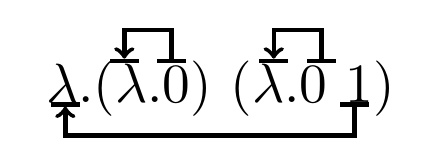
\begin{tikzpicture}[scale=2, every node/.style={transform shape}]]
        \node (term) at (0,0) {$\lambda.(\lambda. 0)~(\lambda.0~1)$};
        \draw[|->|, ultra thick] ([xshift=-10.9pt,yshift=6pt]term.south east) -- ([yshift=0pt,xshift=-10.9pt]term.south east) -- ([xshift=7pt,yshift=0pt]term.south west) -- ([xshift=7pt, yshift=6pt]term.south west);
        \draw[|->|, ultra thick] ([xshift=-8.9pt,yshift=-4pt]term.north) -- ([xshift=-8.9pt, yshift=2pt]term.north) -- ([xshift=-17.4pt, yshift=2pt]term.north) -- ([xshift=-17.4pt, yshift=-4pt]term.north);
        \draw[|->|, ultra thick] ([xshift=18.2pt,yshift=-4pt]term.north) -- ([xshift=18.2pt, yshift=2pt]term.north) -- ([xshift=9.6pt, yshift=2pt]term.north) -- ([xshift=9.6pt, yshift=-4pt]term.north);
        \end{tikzpicture}
    \end{center}
    \caption{Grafische Darstellung der \emph{De-Bruijn-Notation}}
        \label{fig:debruijn}
\end{figure}

In De-Bruijn-Notation sind verschiedene \tlambda-Terme auch für unsere intuitive Gleichheit verschieden, wir benötigen somit keine $\alpha$-Äquivalenz. Substitution, \tbeta-Reduktion, \teta-Reduktion, \teta-Expansion, sowie die Typisierung lassen sich analog zu den üblichen \tlambda-Termen definieren. Wir werden in \Cref{ch:coq} diese Relationen explizit definieren.